% =====================================================================================
%  THE HOLONET MACHINE -- A COMPLETE BLUEPRINT
%
%  Compile:  tectonic holonet_machine_blueprint.tex
%  Engine on this machine: C:\Users\wiljd\tools\tectonic\tectonic.exe
%
%  This document is written to be read two ways at once.  Every section opens with a
%  plain-language explanation that assumes no engineering background, and then gives the
%  exact statement, the measurement, and the command that reproduces it.  A reader who
%  skips every grey box still understands the machine; a reader who reads only the grey
%  boxes gets the specification.
%
%  Every number in this document is measured or proved.  Nothing is estimated.  Where a
%  figure was WRONG in earlier work, the wrong figure is printed next to the right one,
%  because how a number was wrong is part of what makes the right one trustworthy.
% =====================================================================================

\documentclass[11pt,a4paper]{article}

\usepackage[margin=2.4cm]{geometry}
\usepackage{amsmath,amssymb,amsthm}
\usepackage{booktabs}
\usepackage{tikz}
\usepackage{xcolor}
\usepackage{graphicx}
\usepackage{enumitem}
\usepackage{fancyhdr}
\usepackage[colorlinks=true,linkcolor=blue!55!black,urlcolor=blue!55!black,
            citecolor=blue!55!black]{hyperref}

\usetikzlibrary{arrows.meta,positioning,fit,backgrounds,calc,shapes.geometric,
                decorations.pathreplacing,decorations.pathmorphing,patterns,
                trees,shapes.misc}

% ---- palette -------------------------------------------------------------------------
\definecolor{ink}{HTML}{1A1A1A}
\definecolor{past}{HTML}{2E6F9E}
\definecolor{future}{HTML}{B5651D}
\definecolor{plainbg}{HTML}{F4F1EA}
\definecolor{specbg}{HTML}{EAF0F4}
\definecolor{warnbg}{HTML}{F7EDE9}
\definecolor{rule}{HTML}{8A8A8A}
\definecolor{good}{HTML}{2F6B3C}
\definecolor{bad}{HTML}{9E2B25}

% ---- boxes ---------------------------------------------------------------------------
\newcommand{\boxrule}[1]{%
  \par\vspace{2pt}\noindent\colorbox{#1}{\parbox{\dimexpr\linewidth-2\fboxsep}{\strut}}%
  \par\vspace{-2pt}}

\newenvironment{plain}[1][In plain language]
  {\par\medskip\noindent\begin{tikzpicture}
     \node[fill=plainbg,rounded corners=2pt,inner sep=8pt,text width=\dimexpr\linewidth-20pt]
     (B) \bgroup\textbf{\small #1.}\itshape\small}
  {\egroup;\end{tikzpicture}\par\medskip}

\newenvironment{spec}[1][Exactly]
  {\par\medskip\noindent\begin{tikzpicture}
     \node[fill=specbg,rounded corners=2pt,inner sep=8pt,text width=\dimexpr\linewidth-20pt]
     (B) \bgroup\textbf{\small #1.}\small}
  {\egroup;\end{tikzpicture}\par\medskip}

\newenvironment{gotwrong}[1][What we got wrong, and how we know]
  {\par\medskip\noindent\begin{tikzpicture}
     \node[fill=warnbg,rounded corners=2pt,inner sep=8pt,text width=\dimexpr\linewidth-20pt]
     (B) \bgroup\textbf{\small #1.}\small}
  {\egroup;\end{tikzpicture}\par\medskip}

\newcommand{\headline}[1]{%
  \par\medskip\noindent\begin{tikzpicture}
    \node[draw=ink,line width=0.9pt,rounded corners=1pt,inner sep=9pt,
          text width=\dimexpr\linewidth-22pt,align=center] {\bfseries #1};
  \end{tikzpicture}\par\medskip}

% Typewriter text that INHERITS the surrounding size.  Hard-coding \small here made
% filenames inside a \scriptsize table larger than the table itself, which is what the
% last two overfull boxes in this document were.
\newcommand{\cmd}[1]{{\ttfamily #1}}

% Dirac notation, defined locally so the document has no package dependency beyond
% what tectonic ships by default.
\newcommand{\ket}[1]{\left|#1\right\rangle}
\newcommand{\bra}[1]{\left\langle#1\right|}
\newcommand{\braket}[2]{\left\langle#1\middle|#2\right\rangle}

\pagestyle{fancy}\fancyhf{}
\lhead{\small\itshape The Holonet Machine --- Blueprint}
\rhead{\small\thepage}
\renewcommand{\headrulewidth}{0.3pt}

\title{\vspace{-1.4cm}\Huge The Holonet Machine\\[4pt]
       \large A complete engineering blueprint for a computer\\
       whose wiring diagram is a piece of finite geometry\\[10pt]
       \normalsize Every figure in this document is measured or proved.}
\author{\normalsize W(3,3)--E$_8$ project, glue track}
\date{\normalsize 3 August 2026 \quad$\cdot$\quad Passes 2700--2824}

\begin{document}
\maketitle
\thispagestyle{fancy}

\begin{abstract}
\noindent
This is an executable design document for a computer that does not yet exist. Every
promoted statement is classified as \emph{proved}, \emph{simulated}, \emph{synthesized},
\emph{placed}, \emph{published}, \emph{modelled}, or \emph{open}; component evidence is
never silently promoted into an end-to-end machine claim. The logic substrate is the
$40$-point geometry $W(3,3)$. A minimal frame-control core uses \textbf{four operations
encoded by two opcode bits}, while the public eight-opcode three-bit ISA remains a
convenience shell. A new support-first codec maps the $40$ ternary projective points onto
the $15$ nonempty binary tetrahedral masks with exact fiber profile $(4,12,16,8)$, then
leaves a $25$-dimensional within-fiber phase residual. The deep $M_{36}$ grade is proved
two-copy fidelity-distillable under full logical Clifford decoding, with an explicit
branch improving throughout its complete magic-witness interval. That theorem is not an
asymptotic-yield result or a fault-tolerant injection threshold. A published photonic
qutrit \textsc{sum} component reaches $0.92\pm0.01$ fidelity, but that is not a measured
Holonet. This document gives the semantics, datapath, resource evidence, release gates,
and the exact record of claims that failed under stronger tests.
\end{abstract}

\vspace{-4mm}
\tableofcontents
\newpage
% =====================================================================================
\section{How to read this document}
% =====================================================================================

This document has two readers in mind and does not compromise for either.

\begin{center}
\resizebox{\linewidth}{!}{%
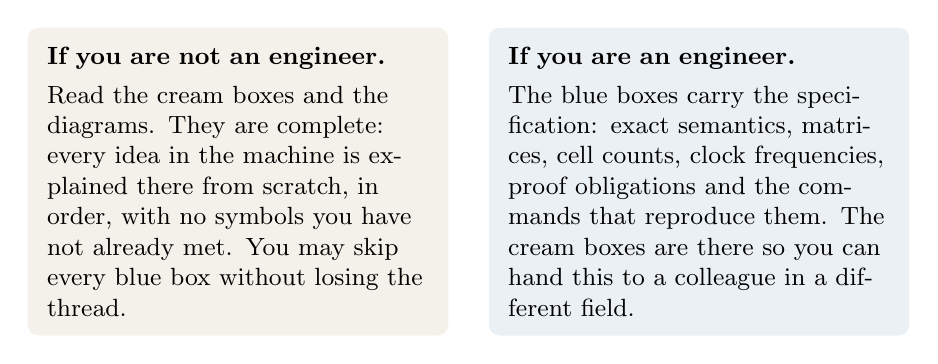
\begin{tikzpicture}[node distance=4mm]
  \node[fill=plainbg,rounded corners,inner sep=7pt,text width=0.40\linewidth,
        font=\small] (a)
    {\textbf{If you are not an engineer.}\\[3pt]
     Read the cream boxes and the diagrams. They are complete: every idea in the
     machine is explained there from scratch, in order, with no symbols you have not
     already met. You may skip every blue box without losing the thread.};
  \node[fill=specbg,rounded corners,inner sep=7pt,text width=0.40\linewidth,
        font=\small,right=5mm of a] (b)
    {\textbf{If you are an engineer.}\\[3pt]
     The blue boxes carry the specification: exact semantics, matrices, cell counts,
     clock frequencies, proof obligations and the commands that reproduce them. The
     cream boxes are there so you can hand this to a colleague in a different field.};
\end{tikzpicture}}
\end{center}

\noindent A third kind of box appears throughout:

\begin{gotwrong}
These record something this project believed, published, and then had to withdraw ---
with the measurement that overturned it. There are thirteen of them. They are not
apologies; they are the reason the other numbers in this document can be trusted. A
blueprint with no errata is a blueprint nobody has checked.
\end{gotwrong}

% =====================================================================================
\section{The machine in one page}
% =====================================================================================

\begin{plain}
Every computer you have used stores information as \emph{bits} --- switches that are
either off or on. This machine stores information in \emph{qutrits}: units with three
settings instead of two. That sounds like a small change. It is not, because of what the
three settings let you do with \emph{geometry}.

Here is the strange and central fact. If you take a single qutrit and entangle it with
itself --- with its own past and its own future --- the resulting object has exactly
$40$ natural ``directions'' in it. Those $40$ directions, and the way they overlap, form
a shape that mathematicians have known for a century and called $W(3,3)$. The machine we
are describing does not \emph{use} that shape as a convenience. The shape \emph{is} the
machine: its memory layout, its instruction set, its network topology, and its error
model are all readings of the same $40$-point object.
\end{plain}

\headline{One qutrit, entangled with its own past, is enough to generate the entire
substrate. The $40$ points of $W(3,3)$ are not $40$ things --- they are $40$ views of
one thing.}

\begin{spec}[The machine, specified]
\smallskip{\footnotesize
\begin{tabular}{@{}p{3.0cm}p{7.6cm}@{}}
\toprule
\textbf{Logical substrate}    & $W(3,3)$: the symplectic generalised quadrangle of order
                                $(3,3)$. $40$ points, $40$ totally isotropic lines,
                                collinearity graph $\mathrm{SRG}(40,12,2,4)$. \\
\textbf{State}                & One qutrit pair $(\text{past},\text{future})$ living in
                                $\mathbb{C}^9=\mathrm{End}(\mathbb{C}^3)$. \\
\textbf{Tracked quantity}     & Four-trit Pauli frame $(x_p,z_p,x_f,z_f)$; decoded first
                                into $15$ binary supports, then an internal ternary phase. \\
\textbf{Minimal frame core}   & Four operations, two opcode bits: $F_p$, both
                                controlled-add directions, and one translation. \\
\textbf{Public ISA}           & $\mathcal{I}_{\mathrm{holo}}$, eight three-bit opcodes;
                                the extras are scheduling conveniences, not additional
                                frame expressivity. \\
\textbf{Group generated}      & $\mathrm{ASp}(4,3)=\mathbb{F}_3^4\rtimes\mathrm{Sp}(4,3)$,
                                order $81\times 51840=4{,}199{,}040$ \emph{exactly}. \\
\textbf{Arithmetic unit}      & Public convenience frame unit: $72$ iCE40 logic cells,
                                $60.80$\,MHz (measured, \S\ref{sec:budget}); the minimal
                                two-bit unit has an independent hardware gate. \\
\textbf{Physical layer}       & Time-bin $\times$ frequency-bin photonic qutrits; a
                                two-qutrit \textsc{sum} component is published at
                                fidelity $0.92\pm0.01$, not as an end-to-end Holonet. \\
\textbf{Evidence firewall}    & Proved $\neq$ simulated $\neq$ synthesized $\neq$ placed;
                                promotion requires every gate in \S\ref{sec:evidence}. \\
\textbf{Network}              & $40$-ary fractal; $N_n=40^n$ leaves, routing depth
                                $8n=8\log_{40}N$; the routing code satisfies Kraft
                                equality exactly, so \emph{every} bit string is a legal
                                address. \\
\bottomrule
\end{tabular}}
\end{spec}

\subsection*{The whole system, at a glance}

\begin{center}
\begin{tikzpicture}[
  font=\small,
  layer/.style={draw=ink,rounded corners=3pt,minimum height=13mm,align=center,
                text width=0.86\linewidth,inner sep=5pt},
  tag/.style={font=\scriptsize\itshape,text=rule},
  arr/.style={-{Latex[length=2.4mm]},line width=0.8pt,draw=rule}]

\node[layer,fill=plainbg] (net)  {\textbf{NETWORK}\; ---\; $40$-ary fractal holonet;
      remote \textsc{sum} costs one Bell pair $+$ two classical trits};
\node[layer,fill=specbg,below=5mm of net] (isa) {\textbf{INSTRUCTION SET}\; ---\;
      four-operation two-bit core; eight-opcode public shell; same $\mathrm{ASp}(4,3)$};
\node[layer,fill=plainbg,below=5mm of isa] (frame){\textbf{FRAME UNIT}\; ---\;
      $4$ trits; $15$ support masks $+$ ternary phase; $72$-LC public unit};
\node[layer,fill=specbg,below=5mm of frame] (geo) {\textbf{GEOMETRY}\; ---\;
      $W(3,3)$: $40$ points, $40$ lines, $\mathrm{SRG}(40,12,2,4)$};
\node[layer,fill=plainbg,below=5mm of geo] (phys) {\textbf{PHYSICS}\; ---\;
      one self-entangled qutrit; time bins $\times$ frequency bins};

\draw[arr] (net) -- (isa);
\draw[arr] (isa) -- (frame);
\draw[arr] (frame) -- (geo);
\draw[arr] (geo) -- (phys);

\node[tag,right=2mm of net.east,anchor=west,rotate=0] {\S\ref{sec:network}};
